\section{Bewertung der Effizienz in Bezug auf die Übersichtlichkeit}
\label{ch:Diskussion:Effizienz}

Die Effizienzbewertung erfolgt anhand der Fehlerquote und der benötigten Zeit zur Erfüllung der Aufgaben.

% Zeit
Die Zeiten der Aufgaben aus dem Usability-Test sind signifikant geringer als die des alten Systems (s. \autoref{fig:usability_test:zeit}). Auch die Einzelbewertung der Aufgaben 1 und 2 liefert dieses Ergebnis (s. \autoref{tab:Usability_Test:rohe_Daten}).
Da die Aufgaben 3 und 4 wie im vorherigen Kapitel bereits erwähnt wenig Relevanz haben, werden diese auch hier aus der Betrachtung ausgenommen. \autoref{fig:usability_test:genauigkeit-zeit_alle-richtige} zeigt, dass die Bearbeitungsdauer mit dem Dash\-board in jeder Aufgabe wie erwartet ersichtlich schneller war.
Dennoch zeigt sich anhand der Aufgaben 3 und 4, dass der Wechsel zwischen mehreren Oberflächen mit dem Dash\-board besser gelingt. Obwohl das Dash\-board eine höhere Fehlerquote aufweist, kann es in einem unbekannten Gebiet überzeugen.

\begin{figure}[h]
    \centering
    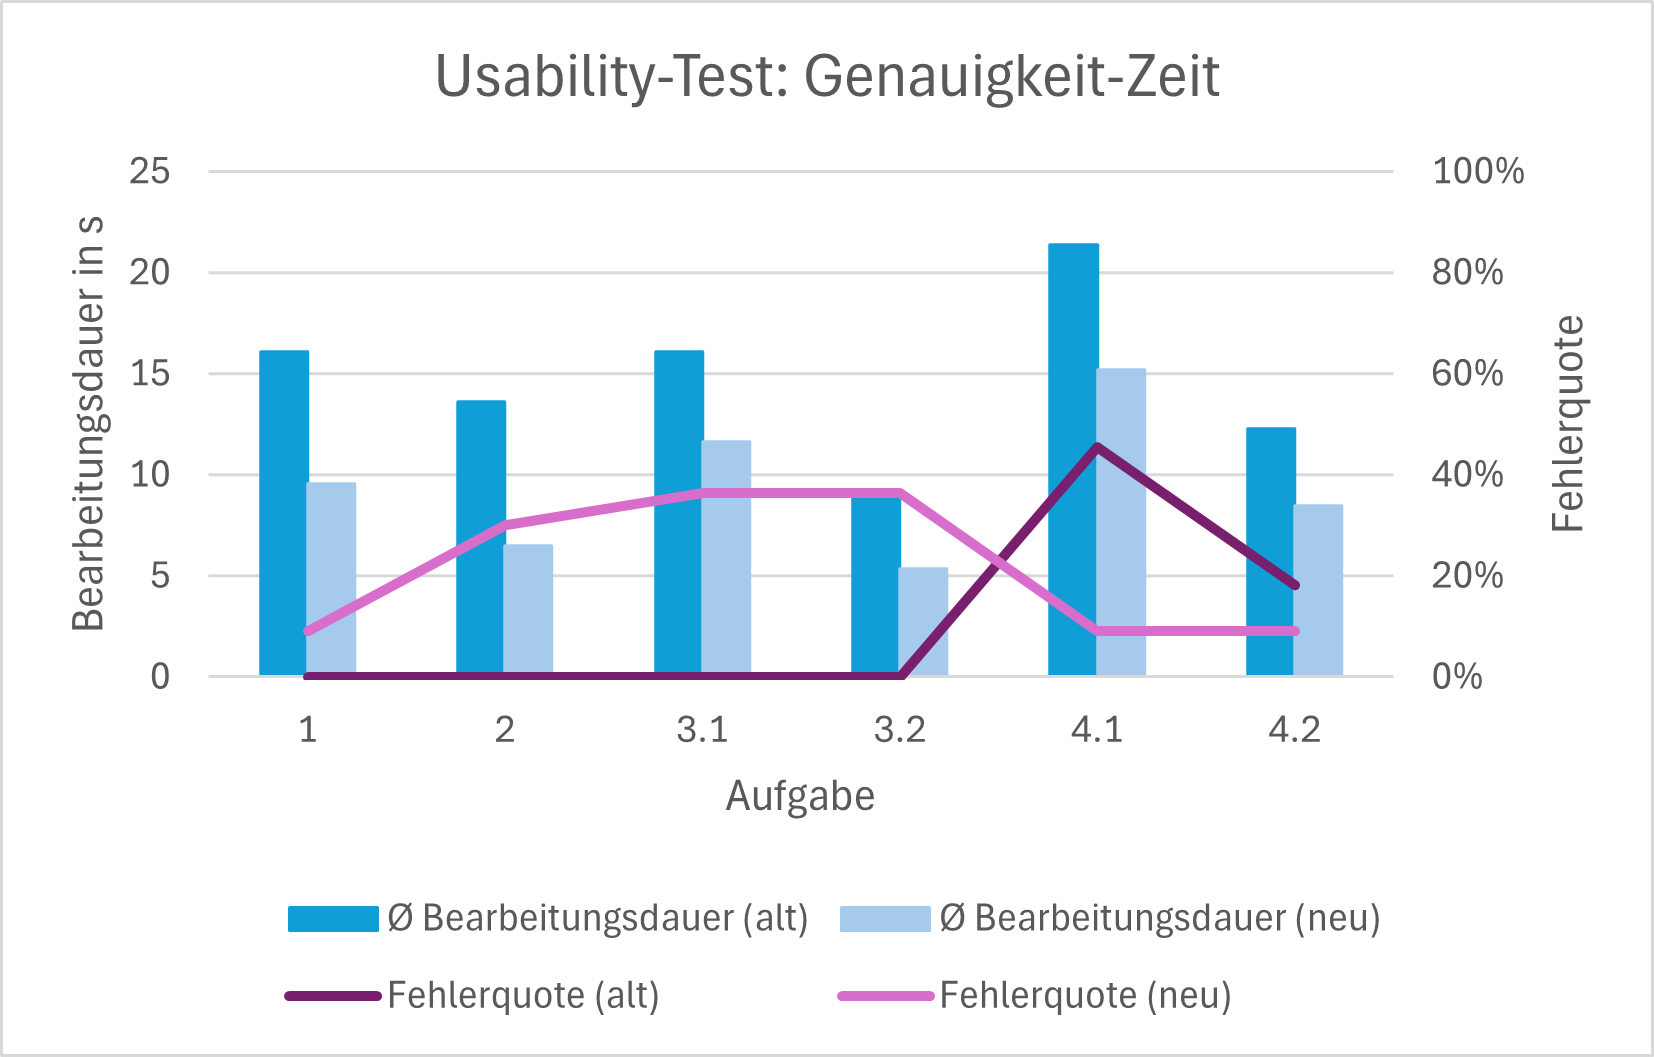
\includegraphics[width=0.8\linewidth]{Diagramme/usability_genauigkeit-zeit_alle.png}
    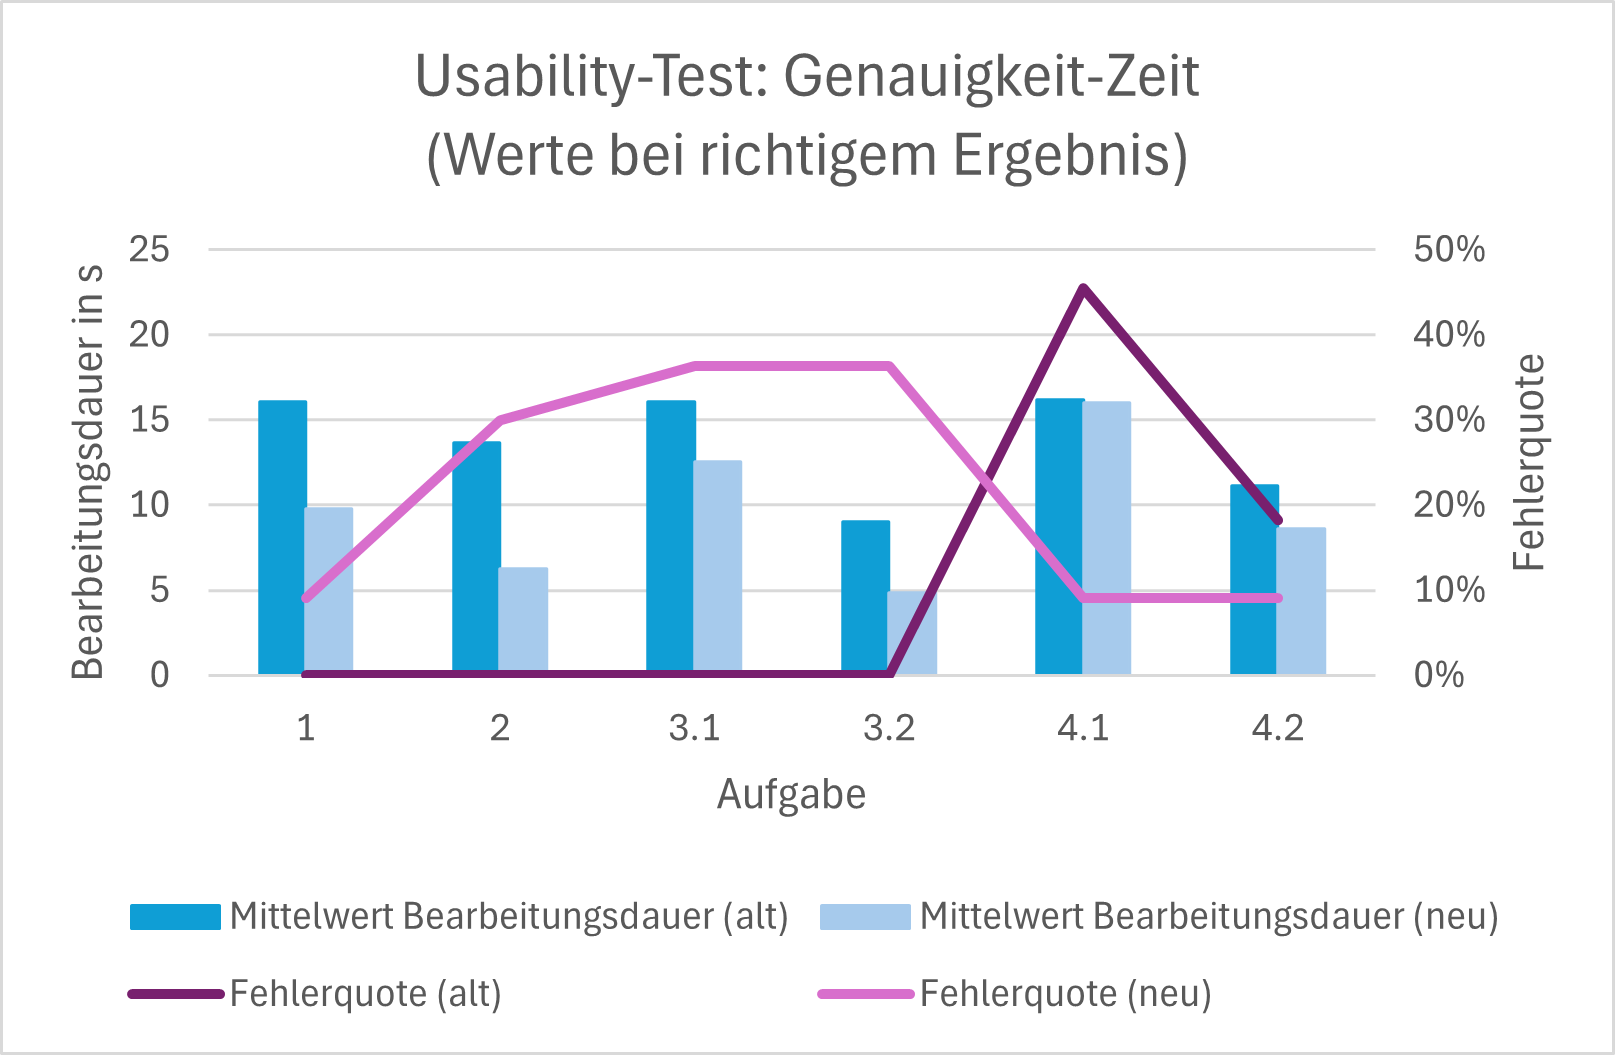
\includegraphics[width=0.8\linewidth]{Diagramme/usability_genauigkeit-zeit_richtige.png}
    \caption{Usability-Test: Zeitvergleich von allen Werten und nur richtigen Antworten - im Verhältnis zur Fehlerquote (Daten aus \autoref{tab:usability_test:mittelwerte})}
    \label{fig:usability_test:genauigkeit-zeit_alle-richtige}
\end{figure}

% Gesetz der Nähe
Das Dash\-board orientiert sich an dem proximity compatibility principle (s. \autoref{ch:SdF:UI:sec:menschenzentriertes_Design}), welches besagt, dass zusammengehörige Informationen beisammen darzustellen sind. Die Anzahl der benötigten Schritte wurde mithilfe des Dash\-board minimiert, da die Anzeige von vielen Ergebnissen auf eine Oberfläche reduziert wurde (s. \autoref{ch:Dashboard:sec:Anforderungen_Auswertung}). % TODO: steht das wirklich in der Auswertung der Anforderungen drin? - wenn nein, reinschreiben!!!
Mit der kürzeren Bearbeitungsdauer zeigt sich, dass sich das Zurechtfinden auf einer Oberfläche wie dem Dash\-board leichter scheint, als auf mehreren wie beim alten System, die zudem verschieden aufgebaut sein können.

% Übersichtlichkeit
Durch die Aggregation aller Ergebnisse auf einer Oberfläche und durch die Farbgestaltung ist eine parallele Suche möglich, ob Fehler vorhanden sind (s. \autoref{ch:SdF:UI:sec:menschenzentriertes_Design}).

% Zusammenhang Fehler::Zeit
In \autoref{fig:usability_test:genauigkeit-zeit_alt-neu} ist zu erkennen, dass im alten System die Personen mit Fehlern langsamer waren als die ohne. Im neuen System ist dies umgedreht. Dies lässt sich daran erklären, dass die Personen, die das alte System nicht so gut kannten, länger für die Aufgaben benötigten und tendenziell auch mehr Fehler verursachten.
Obwohl jahrelange Erfahrung vorliegt, ist es potenziell trotzdem schwierig, sich zu merken, welche Information wo zu finden ist, zumal das alte System aus vielen Abkürzungen besteht.
Da jedoch niemand das neue Dash\-board kannte, lässt sich reininterpretieren, dass die Anzeige etwas genauer untersucht wurde, bevor die Person zum Ergebnis gelang. Die Monotonie des Monitorings scheint noch nicht eingetreten zu sein (s. \autoref{ch:SdF:UI:sec:menschenzentriertes_Design}).

% Genauigkeit-Zeit
\begin{figure}[h]
    \centering
    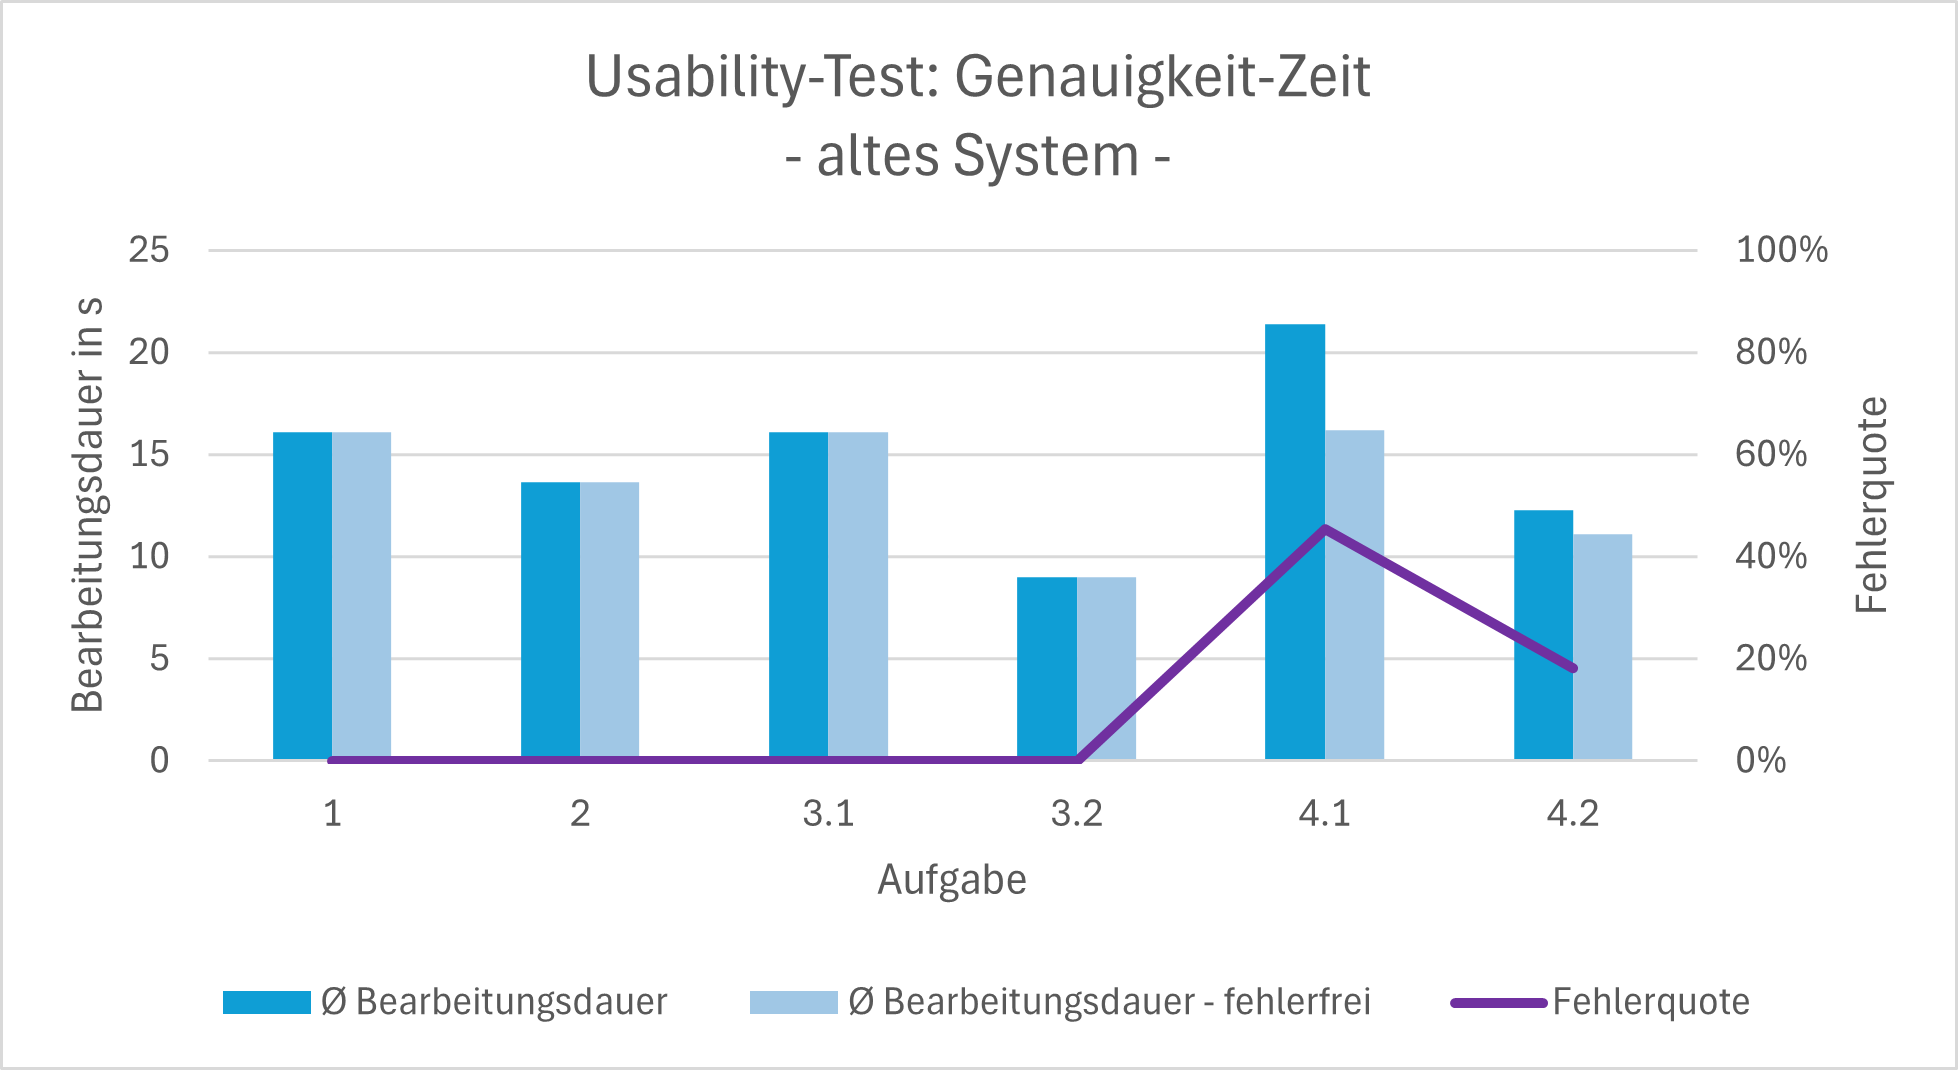
\includegraphics[width=0.8\linewidth]{Diagramme/usability_genauigkeit-zeit_alt.png}
    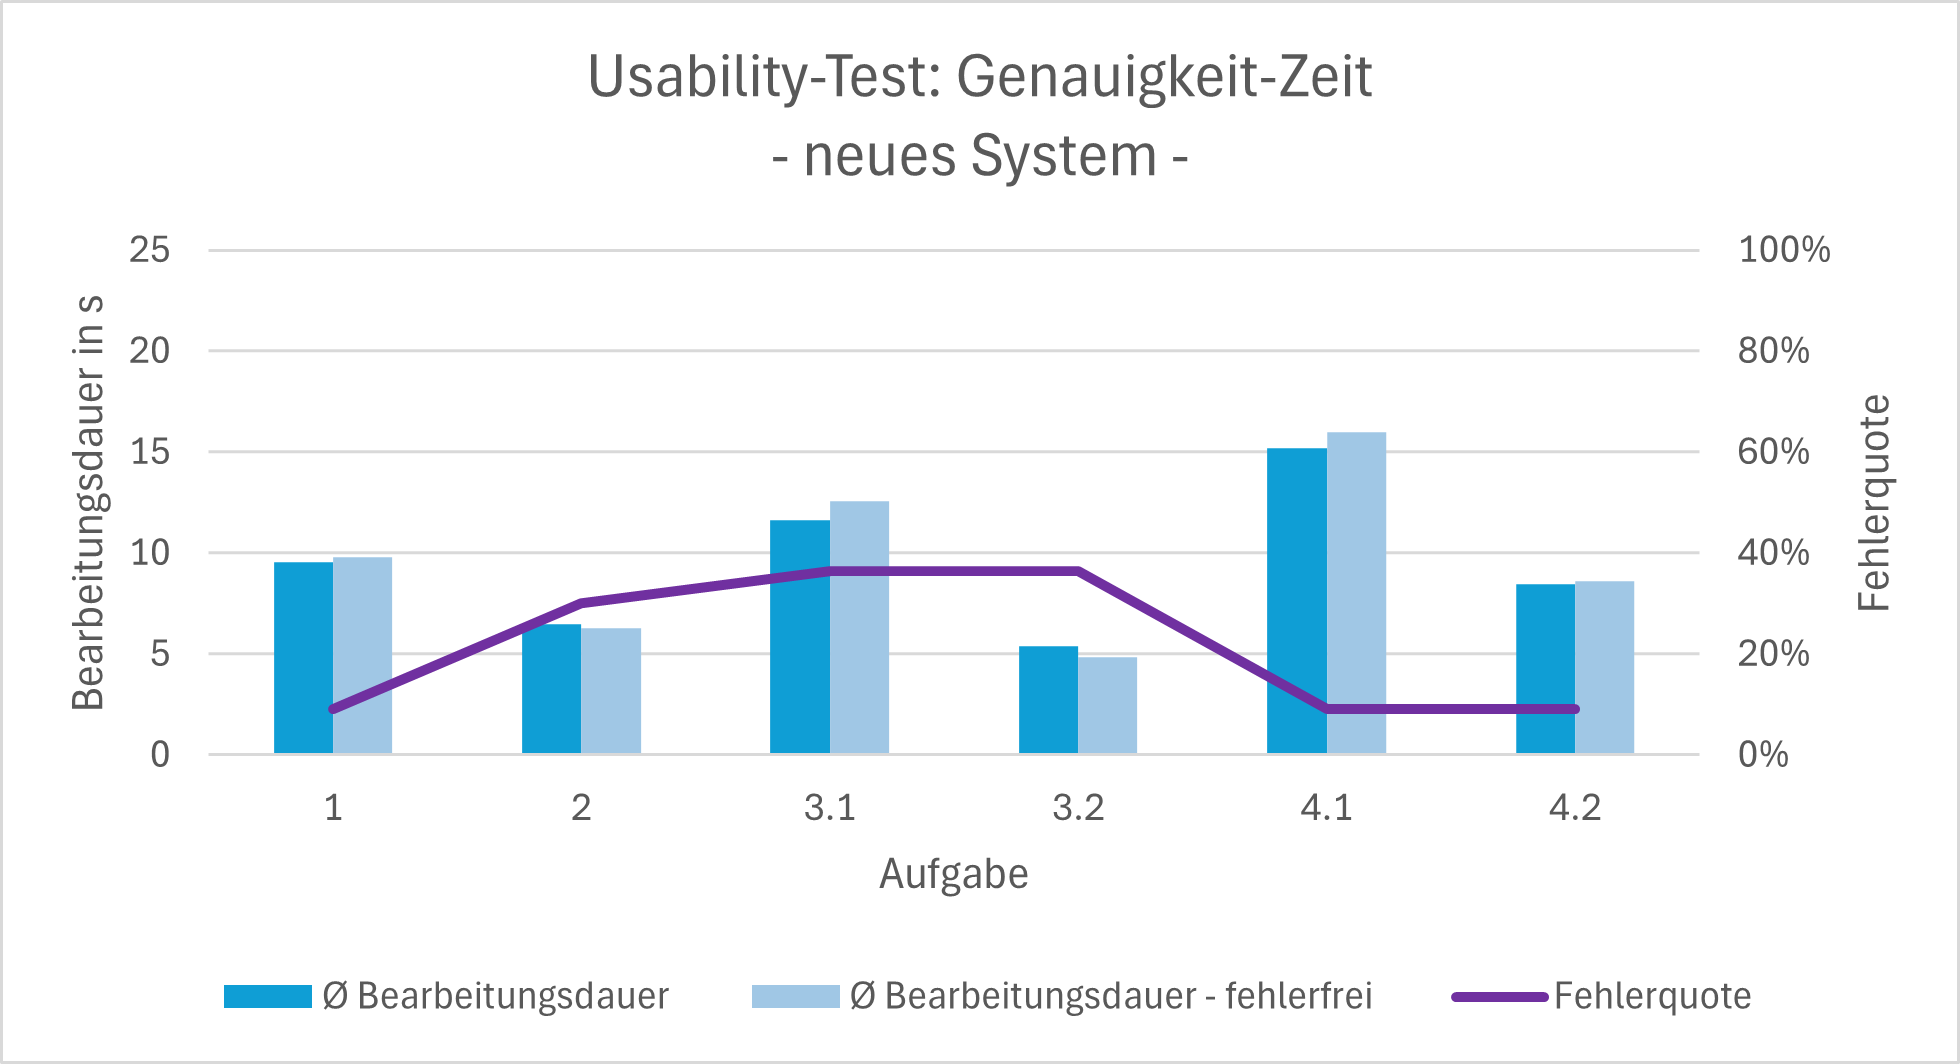
\includegraphics[width=0.8\linewidth]{Diagramme/usability_genauigkeit-zeit_neu.png}
    \caption{Usability-Test: Vergleich Genauigkeit-Zeit im alten und neuen System (Daten aus \autoref{tab:usability_test:mittelwerte})}
    \label{fig:usability_test:genauigkeit-zeit_alt-neu}
\end{figure}

\noindent
Die Daten zur Fehlerquote und Bearbeitungsdauer wurden zu einem Effizienzwert verrechnet (s. \autoref{fig:usability_effizienz}).
Obwohl das Dash\-board im Mittel knapp 50\% effizienter ist, konnte anhand der einzelnen Effizienzwerte kein signifikanter Unterschied festgestellt werden (s. \autoref{tab:usability_test:effizienz}), wodurch die Hypothese $H_{12}$ initial verworfen wurde. Allerdings fällt auf, dass die Effizienzwerte stark schwanken.
Aufgabe 3.1 hat im alten System zwar eine durchschnittliche Zeit und keine Fehler, allerdings sind es im neuen System die zweithöchsten Werte beider Maße (s. \autoref{fig:usability_test:genauigkeit-zeit_alt-neu}). Aufgabe 3.2 zeigt lediglich einen leicht besseren Wert an, da die Zeitdifferenz kleiner ist als bei Aufgabe 3.1.
Aufgabe 4.1 überzeugt mit einem stark positiven Wert. Durch die Umkehrung der Fehlerquote sowie der geringeren Bearbeitungsdauer kann das Dash\-board anhand der Zählaufgabe überzeugen. Der Wert von Aufgabe 4.2 ist etwas geringer, da eine geringere Zeit- und Fehlerdifferenz vorliegt, jedoch das grobe Verhältnis zu Aufgabe 4.1 übereinstimmt.
Die Aufgaben 1 und 2 spiegeln auch die Ergebnisse von zuvor wieder. Da das Dash\-board mit starken Zeitwerten und einer leichten Fehlerquote überzeugen kann. Diese beiden relevanten der Aufgaben können darüber hinaus einen signifikanten Unterschied der Zeitmittelwerte und der Effizienz feststellen (s. \autoref{tab:Usability-Test:ttest_1+2}).

Auf dessen Grundlage der objektiven Werte kann die Hypothese $H_{02}$ nun verworfen werden.

%           Effizienzdiagramm 6.8
% **********************************************
%A1 und A2 - relevant und spigeln die Ergebnisse von vorher wieder --> mit neuem Durschnitt und ttest weiterhin signifikant
%A3 ist negativ, da:
%  --> alt: vegleichbare zeit, gleiche Fehlerquote (zu 1/2)
%  --> neu: zweithöchster Wert in Zeit und Fehler, die anderen haben entweder oder
%A3.2 ist nicht viel besser in ...
%A4.1 drastischer Fehleranstieg in alt --> reduktion in neu
%A4.2 ähnliche zeit, weiterhin niedrigere Fehlerquote

\begin{table}[h]
    \centering
    \begin{tabular}{|l|c|c|c||c|}
    \hline
        Aufgabe 1 + 2 & $\varnothing_{t\_alt}$ & $\varnothing_{t\_neu}$ & t-Test über $\varnothing_t$ & t-Test über Effizienzwerte \\ \hline
        Werte & 14,86 & 8,02 & 0,0137 & 0,0395 \\ \hline
        %Werte & 14,86 & 8,02 & 0,013739065 & 0,039506655 \\ \hline
    \end{tabular}
    \caption{Usability-Test: Zeitmittelwerte und Signifikanzauswertung der Aufgaben 1 und 2 (Weiterverarbeitung der Daten aus \autoref{tab:Usability_Test:rohe_Daten}, \autoref{tab:usability_test:effizienz})}
    \label{tab:Usability-Test:ttest_1+2}
\end{table}

\noindent
Da die Hypothese $H_{12}$ aus subjektiver Sicht bereits zuvor und aus objektiver Sicht nachträglich bestätigt werden konnte, können auch hier die objektiven Daten die Einschätzung und Empfindungen der Nutzer stützen.
